
\documentclass{sig-alternate}
\usepackage{mdwlist}
\usepackage{url}
\usepackage{subcaption}

\begin{document} 

\title{DeepBLE - Localized navigation using Low Energy Bluetooth}
\subtitle{Dept. of CIS - Senior Design 2013-2014\thanks{Advisor: Boon Thau Loo(boonloo@cis.upenn.edu).}}
\numberofauthors{1}
\author{
\alignauthor Eric Kim \\ \email{erkim@seas.upenn.edu} \\ Univ. of Pennsylvania \\ Philadelphia, PA}
\date{April 30, 2014}
\maketitle

\begin{abstract}

  \textit{Currently, mobile phones are the primary method of navigation. 
	However, indoor positioning and navigation poses a unique problem
	because the Global Positioning System (GPS) satellites normally
	used to navigate oudoors have limited use indoors. One solution
	is using Wifi access points as anchors, measuring the signal 
	strength and calulating position using trilateration. Indeed, there
	are tools today that provide the framework for such an implementation.
	However, there are certain disadvantages with using Wifi, namely
	that there are heavy setup costs in laying the foundation for Wifi
	position tracking.}

  \textit{This application aims to address this issue by implementing a
	different method of indoor positioning, one that uses the recently
	developed Bluetooth Low Energy (BLE). With the new APIs 
	released by Google, we can now use Bluetooth devices to act as 
	anchors. The key feature of BLE is the lightweight communication
	between devices that allows us to provide just enough context,
	while still being agile and portable. This peer to peer messaging 
	opens up many possibilities, ranging from applications in shopping 
	malls to emergency response situations. The application will 
	demonstrate the simplicity and robustness of BLE, as well as its
	many extendable applications and capabilities. }

  \textit{The relevant code 
	for the application discussed in the article can be found at 
	https://github.com/erkim/DeepBLE}

\end{abstract}

\section{Introduction}
\label{sec:intro}
With the widespread availability of the smart phone, individual navigation
has been refined such that a user can navigate to and from a particular
address. The statrd used today for outdoor navigation relies on GPS
satellites to track the device location. GPS is generally not well suited for
indoor use for two reasons - 1. GPS does not provide a high level of 
accuracy, and 2. the GPS signal breaks down indoors due to line of sight
(LOS). So rather than using GPS satellites, indoor navigation and 
positioning has been accomplished largely through using networks
of nearby "anchors" or waypoints, that have a static known position. 
The most commonly used framework for anchors makes use of Wifi
access points. A device detects a Wifi access point with a unique ID;
once multiple access points are detected, we can triangulate the exact
position of the device. Indeed there are several existing companies
that will set up the neccessary pieces to allow for step by step navigation
through a shopping mall or departmental store.
\footnote{ See meridianapps.com and senionlab.com}

Google and Apple have both introduced a technology called Low Energy
Bluetooth, also known as BLE or Bluetooth Smart, into their smartphones
that has opened up a new way to navigate indoors. Apple in their recent
release of iOS7 has included in their APIs a technology called iBeacon
that uses BLE extensively for the purpose of geolocation~\cite{apple}.
Any "beacon" that is set up will be available for general iPhone users to 
navigate with; what makes this technology remarkable is that it uses very 
little energy, as the name suggests, has considerable range, especially
comapred to Wifi, and most importantly, it is lightweight and portable.
Similarily, Android in their recent OS release has implemented APIs
for using BLE as well and although it is has not advanced quite as far as
the Apple technology (primarily due to Google's preference of Near
Field Communication, or NFC), it is well defined enough to develop
upon~\cite{android}. As of writing the writing of this paper, smart phones are shipped
with BLE hardware built in, but only the most recent smart phone
releases have the OS that provides a native API to utilize BLE. Suffice
it to say, leveraging BLE for the purposes of navigation is still in its
early stages.

A method of context free positioning has many important use cases. 
One example is in emergency response situations, where location
awareness is of utmost importance. Existing indoor navigation
solutions rely heavily on installed sensor networks, whereas 
emergency agents are more interested in fully auto-deployable
systems~\cite{renaudin}. The current Wifi implementation
requires Wifi access points, a data service that computes location 
(and keeps track of all the locations at any given point), and a 
location specific context (a blueprint overlay of the building; the
access points cannot transmit any information themselves, and
the phone must overlay the context of its position after it calculates 
its location). Although this may be feasible for shopping malls and 
deparmental stores, it cannot be extended into scenarios where such 
a framework cannot be readily or  cheaply set up. We may be able to 
use pre existing Wifi networks, but without a distributed consensus 
(software to identify the various Wifi networks and translate the signal 
strength data), it cannot be extended to an emergency response 
scenario. In addition, Wifi access points may be unreliable, 
inconvenient, and poorly placed for the situation at hand. With BLE, 
all we need to do is drop a few anchors to detect devices, where
they can communicate small pieces of data to each other,
and we can successfully track location.

Current positioning systems are too inflexible; they are neither
portable nor easy to set up. In addition, particularly with Wifi,
a key feature that is lacking is scalability. The field in which navigation
is possible is entirely restricted by where Wifi access points can
be placed. This is clearly a larger issue outdoors, where it may not
be feasible nor particularly cost effective to place Wifi access points
just for the purpose of navigation. Herein lies the fundamental
problems of current navigation - although they take advantage of current 
frameworks and systems already in place, they are entirely bound
by these frameworks. Any issues that may arise must always take
into consideration that these frameworks are unaccomodating; one
cannot alter the GPS network because a particular location gets
bad reception, nor can one freely alter the Wifi access point network
to more convenient locations conducive to position tracking. To tackle 
these inflexibilities, we explore the usability and robustness of BLE 
with a simple app designed specifically to take advantage of BLE's low
cost, portability and easy setup, and its rising ubiquity as
leverage against the Wifi and GPS based positioning systems in 
place today. We address the issue of scalability, portability, and 
robustness all at once by making full use of the lightweight,
grassroots nature of Bluetooth. Issues of line of sight (LOS), signal
reception, accuracy, scalability, can all be addressed by freely
altering the Bluetooth anchor network, either manipulating the 
individual anchors or simply adding more.

BLE is not without its disadvantages however. Since an individual
anchor in a BLE network works with a much smaller scale, LOS
has a much bigger impact on a single device than it would on Wifi
or GPS. For this reason, we depart from the traditional step by
step navigation that characterizes the other frameworks. Instead
the anchors act much more like waypoints, points of fixed location
with enough information about its own location to "point" a user
to the right direction. We will cover this in greater detail in the
System Implementation details; suffice it to say, with BLE, it
is neither desirable nor the most effective to calculate accuracy
to 1 meter or less, like the other implementations do. Another 
important issue is the security between devices; Bluetooth anchors
advertise their information, and it is possible to replicate this behavior,
or manipulate the information. We will discuss possible approaches
and solutions to address this. Finally, BLE is a relatively new 
technology, with only the more recent smart phones built with the
hardware. The APIs are still under development, and the implementation
will be ever changing in the next few years.


\section{Related Work}
\label{sec:related_work}
Fully functional indoor navigation apps, although a relatively recent
innovation, have been implemented before. For example, the 
company SenionLab provides a way for third parties, primarily 
shopping malls and departmental stores, to integrate
an indoor navigation API to their existing applications~\cite{senion}
\footnote{SenionLab: The website contains a splendid video demon- 
strating the capabilities of their turn by turn navigation http://senionlab.com}. 
The API includes location based advertising, allowing for
companies to send tailored advertisements to the customers that
walk by their store, location analytics, the ability to gather data on 
user behavior, and most importaantly, a fully functional step by step
navigation system that works at the granular level. As discussed
previously, these apps rely on Wifi access points as the anchors.
Although this allows the application to pinpoint the exact location
of the device and track it as it moves, it does not provide 
environmental awareness. These Wifi based implementations
do not carry any data about their particular locations, such as
whether a store carries a particular product, or if the store is
currently having a sale. A fundamental assumption is being made
in this case, that is, users already know \textit{where they want
to go}, rather than \textit{what they want to do}, and this is the
basic issue we seek to resolve.

We cannot forget the costs of implementing a framework that 
uses Wifi access points. Wifi needs to be set up well in 
advanced, and a data service that calculates position must be
implemented. Finally, Wifi has associated costs that the party must
invest in, such as monthly internet charges, maintenance, and an
app for users to download so that all of the positioning has the
correct context and protocols. This is on top of the previously
mentioned weakness of Wifi in general.

With BLE, we no longer have to make this assumption. BLE
singal transmitters are low cost: for example, with Apple's iBeacon, 
"beacons" as the'yre called costs as little as 30 to 40 dollars. As 
the name suggests, BLE uses little energy. Most important of all
they can be ubiquitous - shopping mall where every store has a
proximity sensor, or an anchor, can achieve much more granularity
than Wifi access points could ever provide. With this granularity
comes enriched data - anchors no longer just provide a specific
location, they can provide specialized promotions, tailored 
directions, and more important for our purposes, contextualized
notifications~\cite{gottipati}. This means that a user can
navigate through a room and discover information about their
specific location, such as other users in the room or immediate
area.

Indoor navigation using older Bluetooth technology, Bluetooth
Classic as it is now called, has also been implemented. These
systems compare the signal strengths of surrounding Bluetooth
devices to a database of measurement taken across the indoor 
area, in order to estimate the user's position. Accuracies of
approximately 1.5 meters have been achieved through such
methods~\cite{bekkelien}. Although we will not be implementing 
step by step navigation, as these systems have done, it is certainly 
possible to extend BLE navigation such that we can achieve these 
levels of accuracy. 

Also important to note is that there are certainly companies 
that implement a BLE based positioning system~\cite{indoo.rs}.
Indoo.rs for example, offers a package 
of bluetooth anchors along with and API for navigation. Their 
system involves integrating their SDK with existing applications. 
Features include navigation (not specifically for indoor use, but 
optimized for indoors), routing, and analytics that track user 
movements. The main difference between our application and 
the SDK created by Inddo.rs is that our application aims to be 
completely stand alone, optimized for the emergency response 
use case. Our biggest motivation is to remove the need for setting 
up complex systems in order to start navigating.

The app is developed on Google's Android, and although
the APIs are well founded, Apple's iOS7 has a much more
mature API allowing for more powerful applications of BLE.
As such, the implementation details are Android specific; 
with more capabilities, an iPhone implementing a BLE 
application may behave differently from our application.
Indeed, the previously mention indoor navigation APIs are
optimized for Apple's iPhones.


\section{System Model}
\label{sec:sys_model}

\begin{figure}[h!]
	\begin{center}
		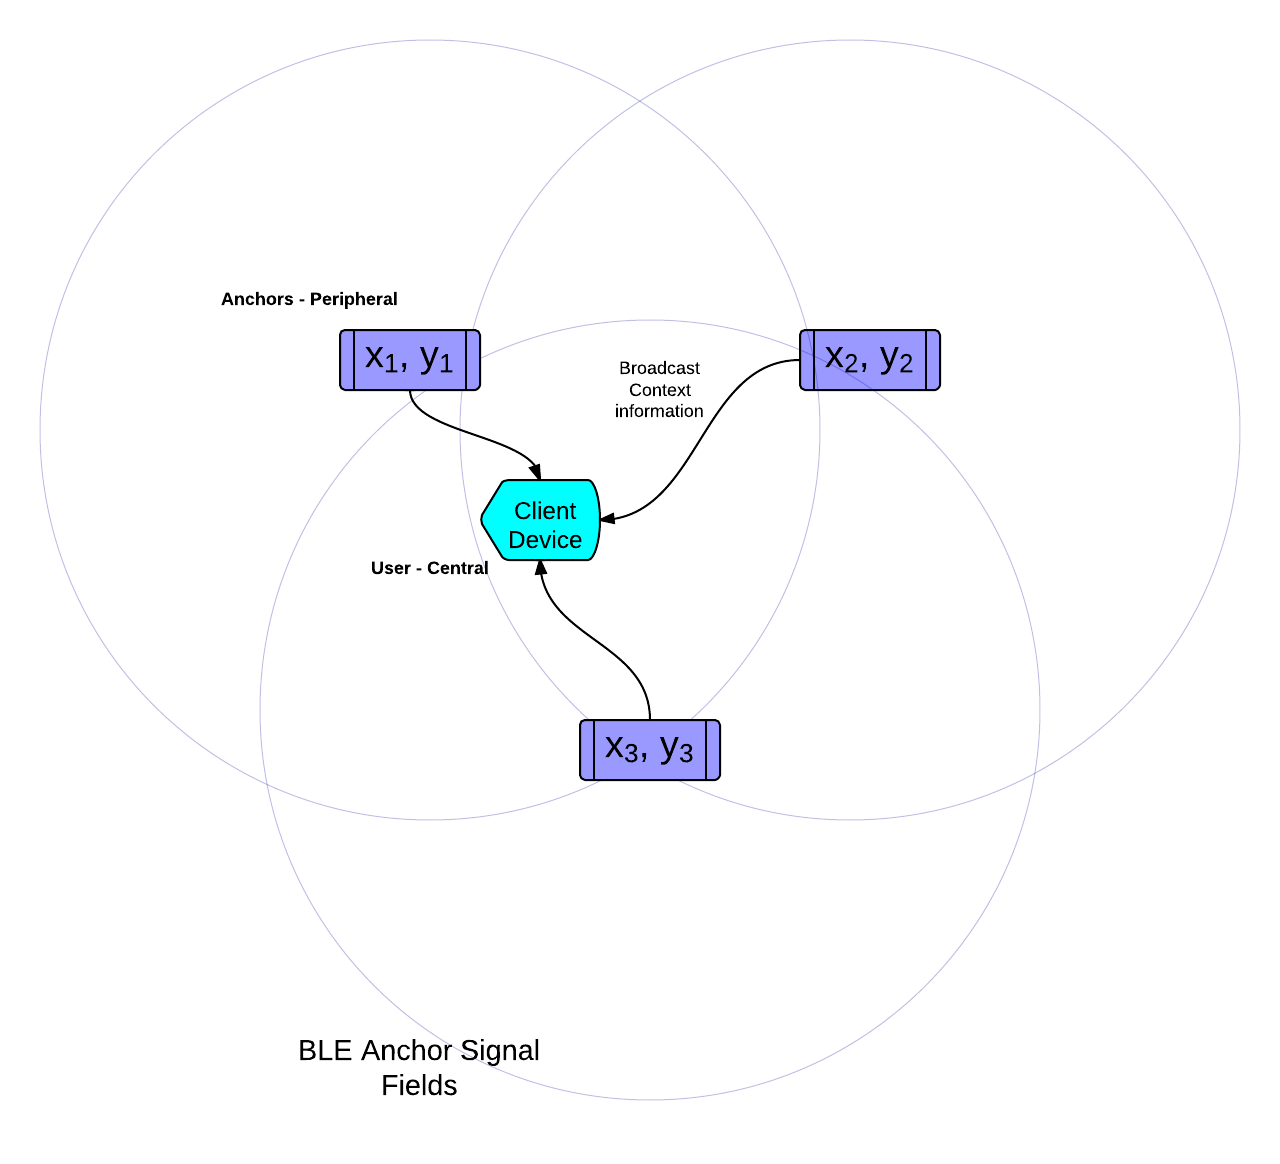
\includegraphics[width=1.00\linewidth]{system_model}
	\end{center}
	\vspace{-12pt}
	\caption{BLE Client Anchor System Model}
	\label{fig:System Model}
\end{figure}

Following our design goals of portability, scalability and 
robustness, our BLE app will provide just enough context
with each anchor, with the primary advantage of being
fully customizable - the user enters information about
the anchor, instead of relying on a predefined context.
Before moving forward, a few details about how the Bluetooth
Low Energy system works must be discussed.

As designed by Bluetooth themselves, BLE centers around 
the use of the Generic Attribute (GATT) Profile~\cite{bluetooth_core}.  
The GATT profile is a general specification for sending and 
receiving short  pieces of data known as "attributes" over an LE link. 
This profile allows highly customizable applications suited for their 
individual purposes, enabling devices to co-operate predictably in 
particular environments. The attributes are defined by a set of 
services and characteristics. Services and the characteristics 
associated with them are essentially tailored protocols for 
communication for certain devices. For example, the link loss 
service defines behavior when a link is lost between two devices. 
This service consists of a single  characteristic, the alert level 
characteristic. Each characteristic contais a single value, with any 
number of descriptors describing the characteristic. In our example, 
the alert level characteristic carries an indication on how devices 
should behave when a link is disconnected. Important to note is 
that there is an extensive list of predefined servies and 
characteristics available for most common applications, and in 
addition, custom services and characteristics may be defined, 
either through a generic attribute service, or a developer defined 
service.

The GATT profile defines a server client relationship between
devices. The server acts as a database, holding information about
the device, whether it be it's current coordinates, or the context
in which the device is placed. It stores the data transported 
over the Attribute Protocol, and acceptes Attribute Protocol 
requests, commands and confirmations form the client. It then
sends responses to requests and when configured, send indication
and notifcations asynchronously to the client when specified 
events occur on the server.
It's clear that our anchors will take the server role in this case. 
Complement to the server role is the client role. Client devices 
transmit and receive data to and from the server devices. 
Note that these roles are not necessarily set in stone; the roles are 
interchangeable, and  in the device to device communication case 
in particular, a device takes on both roles. There are other times 
where this is not the case, for example a bluetooth headset with 
no storage capabilities will naturally act as the client, paired to the 
server device. 

\begin{figure}[h!]
	\begin{center}
		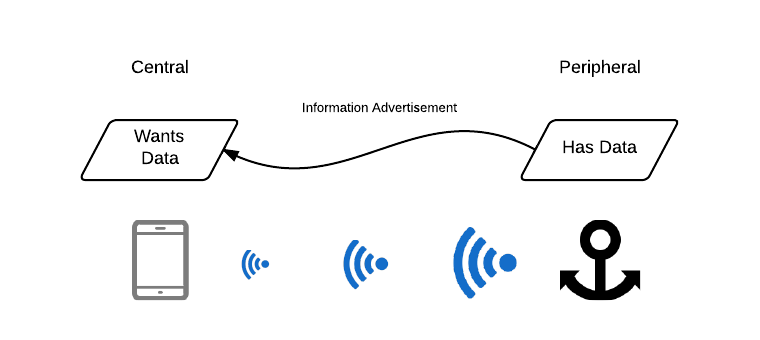
\includegraphics[width=1.00\linewidth]{central_peripheral}
	\end{center}
	\vspace{-12pt}
	\caption{The Central Peripheral Relationship}
	\label{fig:Central Peripheral}
\end{figure}

Unique to Bluetooth Low Energy are the central and peripheral roles.
This relationship is quite similar to the server client relationship,
but now with Bluetooth Low Energy, the peripheral role has 
additional functionality. In addition to being able to store data 
for client devices to retrieve, peripheral devices actively broadcast
the information they carry. This is made possible due to the 
GATT profile; previously for a device to communicate with 
another, it had to "pair", or establish a connection. This 
central peripheral relationship is one of the primary reasons
that BLE consumes the energy it does; no longer is this 
pairing required for two devices to communicate. A
peripheral device can simply broadcast its information,
while central devices in the area can collect that data. The
important innovation to note here is that a device no longer
has to maintain a constant link between another to receive
or transmit data. By following the protocols of the GATT profile,
devices are now able to quietly collect and advertise data.

For our application, anchors take the server/peripheral role,
containing data about their location and broadcasting information
about their location; specifically, a custom defined service that
holds a string containing some context about the device will 
handle the communication between the anchor and the client
device. User devices take the central role, collecting anchor 
data as they pass through the anchor's bluetooth fields. 
For our purposes, a device may switch from the client to
the server role, since Bluetooth devices specifically designed
to act as anchors broadcasting their context are out of reach.
To address this, we simply allow for a smartphone to take
the role of an anchor; it is easy to see how one would design
hardware devoted entirely to being an anchor. 

The application provides a user the option to set their device
as an anchor; the device will then sit quietly and allow
other devices to discover it. If not an anchor, a device will 
then be able to scan for other anchors. Once it finds an 
anchor, it will update its own location according to the information
received from the anchor. If there are multiple anchors in range,
the device will connect with whichever anchor the user chooses.
\textit{see figure 1}

Put together, the application will provide users with a simple
interface to connect to anchors as they navigate. Client devices
will scan as they move, picking up location information from each
of the anchors it connects with. This is the basic waypoint navigation
discussed earlier. 

We purposely avoid calculating exact position in our application.
For precise position estimations, the dependence between distance
and received signal strength has to be accurately measured and scaled
accordingly. In addition, particularly indoors, boundary conditions like
reflections and wall damping make the use of the equation for
the free-field propogation impossible. In order to calculate 
exact position, we need precise Received Signal Strength
Indicator (RSSI) measurements~\cite{feldman}. Although Android
allows for easy access to RSSI, we sacrifice scalability and fault
tolerance by having client devices calculate exact positions.

\section{System Implementation}
\label{sec:sys_implement}
Before moving on to the system implementation, some details 
regarding the Bluetooth Low Energy specifications are included. 

\begin{table}[h!]
    \begin{tabular}{ll}
    Technical Specification  & Bluetooth Low Energy ~\cite{bluetooth_core} \\ \hline
    Distance/Range           & >100m (>330ft)              \\
    Over the air data rate   & 1 Mbit/s                          \\
    Application throughput   & 0.27 Mbit/s                    \\
    Security                 & 128-bit AES with Counter     \\ 
			        & Mode CBC-MAC, user         \\
			        & defined application layer      \\
    Latency                  & 6ms                                       \\
    Peak current consumption & <15 mA                     \\
    Other info               & Includes message integrity   \\ 
			        & check, adaptive frequency    \\
			        & hopping 
    \end{tabular}
\end{table}

The application has two main parts - a context page, where
a user can define relevant details regarding the device, and
a device scan activity, where anchors are discovered and
connected to. In the context page, the user is able to 
name their device; this is the primary method in which a user
can describe the context of the device. This is most important
when the device is set to act as an anchor. Client devices
that connect to this anchor will recognize this device as 
whatever the user has decided to name the anchor. Since
the context here is a simple string, it is suggested that a 
user inputs something descriptive about where the device
is located. For example, a user can name their anchor
as "home", and all clients that detect and connect with this
anchor will have their current anchor set as "home".

\begin{figure}[h!]
	\begin{center}
		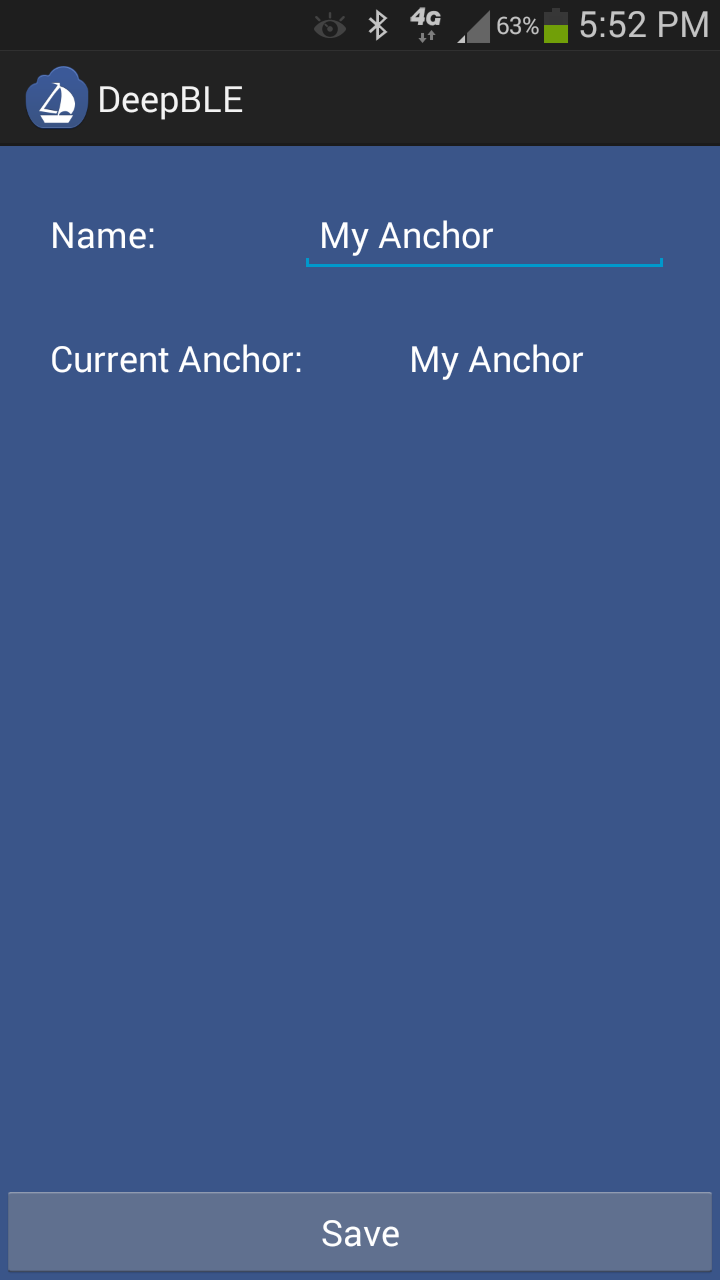
\includegraphics[width=.5\linewidth]{device_context}
	\end{center}
	\vspace{-12pt}
	\caption{The Device Context Activity}
	\label{fig:Device Context}
\end{figure}

A custom GATT profile was designed off of the Generic Access
Profile. Device verification (verifying the device is using the
same GATT protocol) is done using Universally Unique 
Identifiers (UUIDs). The GATT profiles provided by Bluetooth 
all have a UUID that acts as a verification between devices (that
the profile and service in question are relevant). A custom, 
random UUID was generated for our purposes, and on this 
UUID the device context characteristic was defined. This 
characteristic contains the string that the user defined earlier in 
the device context page. Client devices contain a global variable 
called "currentAnchor", which contains the instance of the anchor
that the client device is currently connected to. Client devices
then read the characteristic transmitted by the anchor device,
where it will then appropriately record the information it receives.

\begin{figure}[h!]
	\begin{center}
		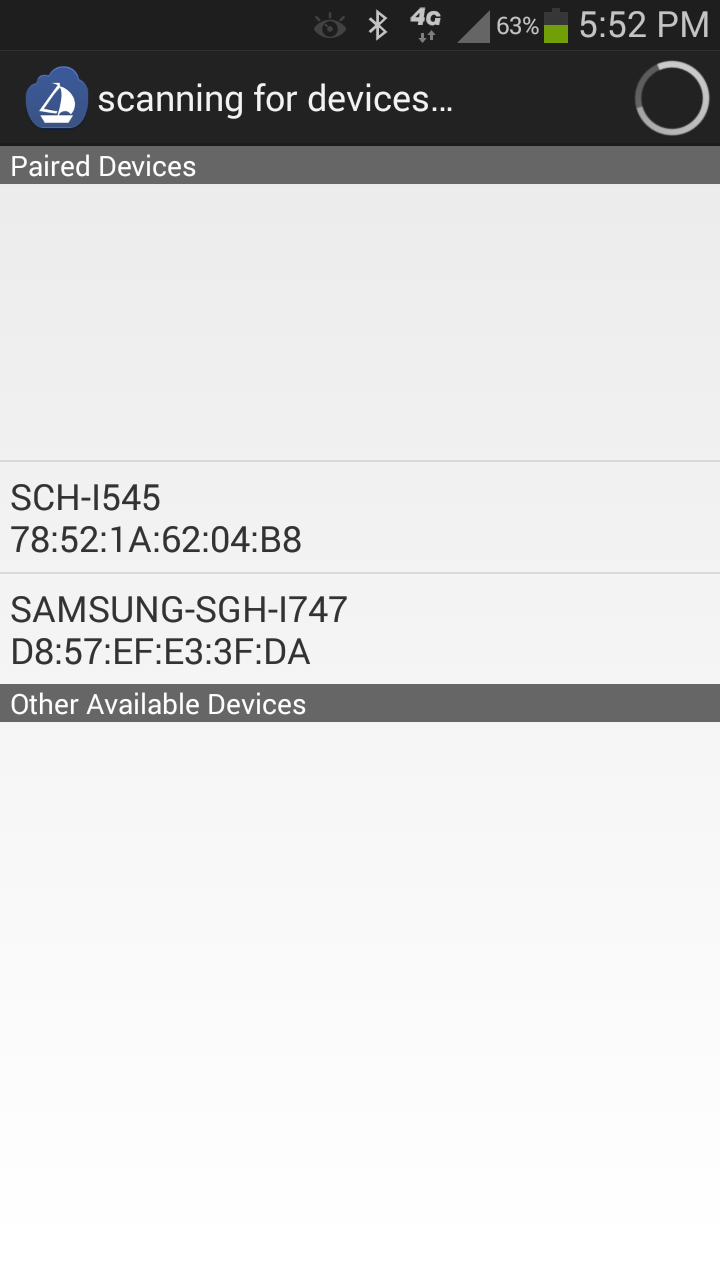
\includegraphics[width=.5\linewidth]{device_scan}
	\end{center}
	\vspace{-12pt}
	\caption{The Device Scan Activity}
	\label{fig:Device Scan}
\end{figure}

On the device scan activity, a search for discoverable devices
can be initiated. To handle this, a separate BluetoothLeService
class was defined to take care of all BLE related services,
which included connecting to a device, writing and reading
characteristics, broadcasting updates, initiating discovery, 
and defining which GATT services are relevant to the device.
Once a scan is initiated, the user will then be able to
choose out of the anchors in the user's range which to 
connect to and gather context from.

The connection and data transfer is implemented using Bluetooth
Classic. Currently, the Android APIs do not support devices
taking the peripheral role; that is, devices cannot yet broadcast
their information and push it down to client devices that are
scanning. This is purely a limitation of the Android APIs, and
it is foreseen that Android will release hardware and software
support for devices to take on the peripheral role. Since
this was the case, Bluetooth Low Energy was not used to
transmit data. Unfortunately, this causes the application to lose
many of the benefits stated earlier associated with Bluetooth
Low Energy. Most importantly, this required a client device 
to pair with an anchor and maintain a channel between which
the devices could transmit and receive data. Characteristics
were still written thanks to the BluetoothLeService class, and
all the appropriate protocols associated with the GATT profile
and followed, but this is not exposed to the user, since in practice
the communication itself is done entirely through Bluetooth
Classic. It should also be noted that, since the device only needs
to maintain connection long enough to receive the context information
from the anchor, the connection does not have to be maintained
for extended periods of time. Once the information is transmitted,
the device promptly disconnects the pairing with the device anchor. 

With the use of Bluetooth Classic, a separate BluetoothService class
was defined to handle the Bluetooth connection. 
Since Bluetooth Classic involves a continuous connection between 
devices, synchrony was of utmost importance. The BluetoothService
class is in many ways similar to the BluetoothLeService, but with
some additional restrictions. All the same function calls, such as
connecting, writing, reading and sending messages, and broadcasting
updates were included and modified to maintain synchrony between
the device it is paired with. Each function call runs as a thread in
parallel with the paired device to maintain synchrony.

\begin{figure}[h!]
	\centering
	\begin{subfigure}{.5\linewidth}
		\centering
		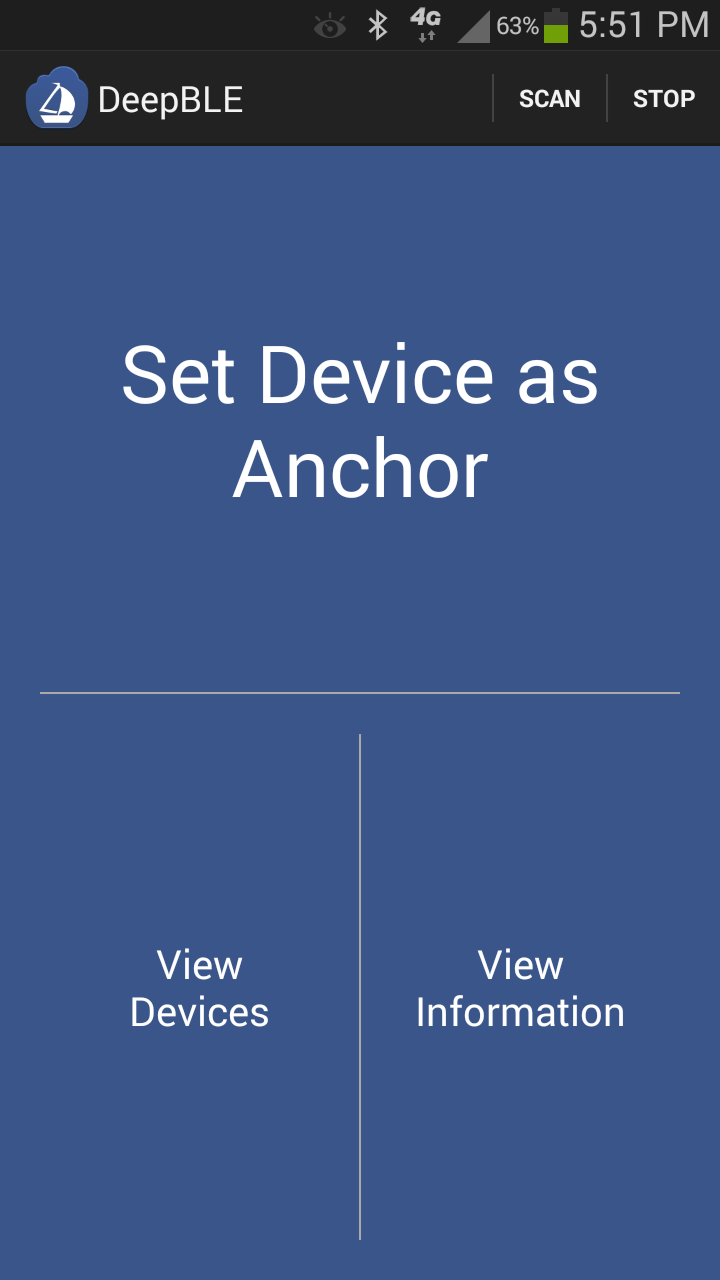
\includegraphics[width=.8\linewidth]{main_activity}
		\caption{Main Screen}
	\end{subfigure}%
	\begin{subfigure}{.5\linewidth}
		\centering
		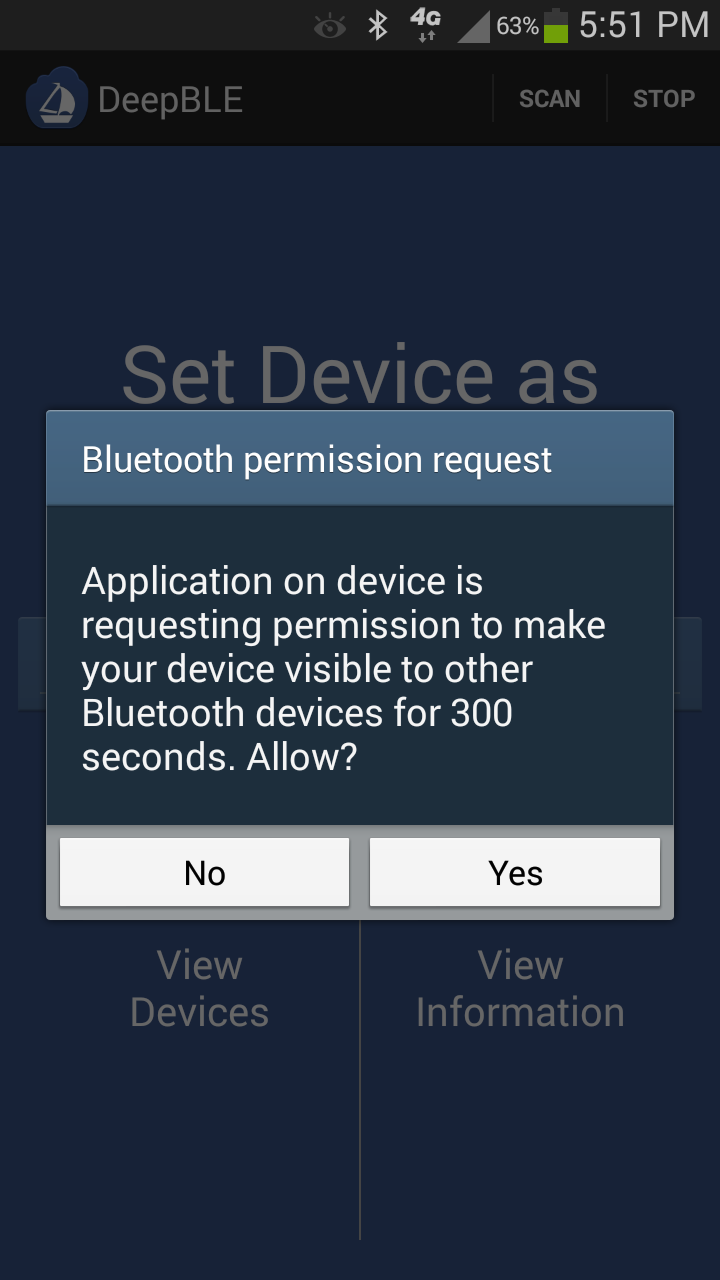
\includegraphics[width=.8\linewidth]{set_discoverable}
		\caption{Set Anchor Prompt}
	\end{subfigure}

	\caption{The Main Anchor Activity}
	\label{fig:Main Activity}
\end{figure}

Controlling these two activities is the main device activity, where a
user has the option to start scans or view and edit their information.
Here, the option to set the device as an anchor is presented. Once
a user decides to set the device as an anchor, the application
ensures that the device becomes discoverable to other devices
for 300 seconds (this is a hard limit set by the Android Bluetooth
API before it requires user input to initiate discoverability again). 
One of the drawbacks of using Bluetooth Classic here is
the energy cost associated with ensuring a device is discoverable;
the device has to broadcast its presence and open up a channel for
other clients to connect with. Due to this, the hard limit of 300 seconds
was imposed by Android, and this further inconveniences the user, forcing
them to reset the device as an anchor every five minutes. This 
introduces a inflexibility of the anchors - a user must reinitiate 
discoverability every 5 minutes. Once Android releases their
APIs for the peripheral role, this will likely not be an issue any longer, 
as a device can remain discoverable for any amount of time using
BLE.

The relevant libraries include the Android Bluetooth Library 
(BluetoothAdapter, BluetoothProfile, BluetoothGatt), and the
Android Library~\cite{android}.
A custom class called ProximityGattAttributes was also defined;
this class contains the custom defined GATT characterisitics
used to describe the anchor context. Also included are the
generated UUIDs on which the service and characteristics 
are built upon.
The protocols and specifications set out by Bluetooth 
were also extensively used~\cite{bluetooth_core}.
The relevant code can be found at 
\\ https://github.com/erkim/DeepBLE

\section{Results}
\label{sec:results}
The application behaved as expected - a user can connect
to a device and initate a pairing, after which the relevant contextual
information was transmitted. 

One of the more interesting results was the device's sensitivity
to LOS. Step by step navigation is indeed inpractical, primarily
due to interuptions in signal strength due to LOS. The triangulation
measurements rely on very minute changes in Received signal 
strength indication (RSSI) to correctly calculate position; when
a device's connection is interrupted by a wall or object, the
calculations result in very erratic position estimations. In addition
Bluetooth classic only allows for one device to be paired at
a time. This prevents the necessary three devices a device
used to triangulate its own position. However, it is possible 
to effectively "reduce" the field of detection of a device. A device
can ignore the signal received from devices outside a 
developer specified range, allowing for more accurate 
location measurements.

The robustness of Bluetooth was made the most apparent; 
it is quick and simple to setup additional devices as anchors
(although in this implementation, due to the reliance of Bluetooth
Classic for data transfer, discoverability must be manually
reinitiated, and therefore it is impractical to setup large
amount of anchors). With the addition of the peripheral role
by Android, it is easy to see how anchors can be placed
freely and judiciously to increase accuracy, fault tolerance,
and effective range. 

A major flaw discovered when implementing the peer to peer
communication was the interference of other devices. Again,
with the use of Bluetooth Classic, we lose the Generic Attribute
Profile associated with Bluetooth Low Energy. One of the 
important jobs of the GATT Profile is to filter out the 
irrelevant devices that are in the area; clearly a user has no
interest in the bluetooth headset a few feet away. Both 
Bluetooth and BLE scans were implemented, and BLE 
was by far the more accessible of the two. Only the devices
carrying the correct GATT profiles were detected, allowing
for the user to easily see which devices are anchors.
In addition, the Bluetooth Classic scans do not allow 
transmission of information without first establishing a 
pairing. The only information made available to other users
during discovery are device names, which in general are 
very unfriendly. As such, it is very difficult for a user to judge 
which devices are anchors without prior knowledge of devices,
relevant or not, in the area. Again, this limitation should be 
lifted when the peripheral role is introduced to Android; without 
a connection requirement, anchors can freely advertise their
presence and information, which the central client devices
can gather according the the GATT protocol.

Inherently with this user inputted context is the lack of 
absolute information. With traditional navigation systems and
a predefined context, direction, absolute position, and 
a rendered map comes naturally. With BLE, we avoid
the use of a global predefined context which overlays
the network. This prevents BLE applications from using more
universal methods of navigation, such as direction or absolute
position. The user must know beforehand what context
the anchors are placed in. For example, in a shopping
mall, it is easy to input as an anchor name a particular
store. The user can see that the anchor corresponds to 
the particular store, and using that information infer 
where they are. There is an inherent reliance on the
users to know where they are with respect to their
surroundings. In addition, there is an assumption
that the anchor's description is actually accurate, or even
easily comprehended by the users! Descriptive and
user-friendly anchor names are suggested; the
application leaves it entirely to the person setting
up the anchor network to decide how the anchors
are described.

Finally, the app sought to test the capabilities of Bluetooth LE,
it did not address issues of security. Since the context
of a location is entirely user defined, a user is free to 
feed misinformation to the anchor, potentially confusing
a user trying to navigate using the existing anchors. To take
this one step further, in the large scale use case, removing
or altering any of the anchors can disrupt the entire
network, which poses problems particularly in the large scale
case, where it may be difficult to identify which anchors
are accurate. The anchors are limited by the 100 meter
range of Bluetooth, and so there is no global communication
between anchors; if one of the anchors fails or is broadcasting
incorrect information, the other devices will independently run
without correcting the issue. To address this, a distributed
consensus protocol must be implemented, as well as method
for anchors to communicate with one another to form a
loose network.

\section{Future Work}
\label{sec:future_work}

One of the primary goals of designing an application that can
effectively use BLE was to demonstrate how the application
could be extended to a wide variety of use cases. The strength
of BLE comes from its scalability; additional anchors are easy
to add to the network, and they seamlessly contribute accuracy,
range and robustness to the network. BLE navigation may
have limited use with two or three anchors, but it immediately gains
strength with the addition of two or more anchors. 

When we enable anchor to anchor communication 
(ideally this will be feasible with the peripheral role), we
open up interesting graph related applications. Namely,
the anchors can contain localized information about
the anchors surrounding them, forming a loosely connected
network of anchors. In the most simple case, the
anchor should not need to maintain constant communication
with the other devices, since the anchors are unmoving.
With some additional information about its immediate
surroundings, we can represent each anchor as a node
in a graph with knowledge of its neighbors and nothing
else. By doing so, we can then implement graph search
algorithms to optimize navigation for client devices.
A new custom GATT profile would be required to implement
this, as the anchors would require a protocol to communicate
with client devices the anchors in its vicinity. Combining
this information, a client device can conceivably navigate
step by step, if the contextual information is tailored for
that purpose. An example of a use case would be ocean
navigation, with various anchors placed on particular
longitude latitude coordinates. If the anchor context is
defined as these coordinates, a client device can navigate
through the various anchors. 

A highly desirable feature to add would be this graphical 
representation of the Bluetooth network, that updates as
the user passes through other anchors. 

With the extensive use of the Bluetooth protocol, it is easy to
integrate the application with existing bluetooth hardware.
An example use case would be Bluetooth navigation to 
aid the visually impaired. With a well designed bluetooth
headset, we can use anchors as waypoints to help
the visually impaired navigate.

Finally, to optimize navigation and allow for large scale
use, dedicated anchors must be designed that will interact
with the application. Using smartphones as anchors is both
inefficient and inpractical. In real life scenarios, anchors
should be durable and portable to see widespread use.

\section{Ethics}
\label{sec:ethics}
The extended application has many commercial and 
non commercial use cases. Any situation where contextual
awareness or navigation is required will find Bluetooth
navigation useful. Due to the portability of Bluetooth, this
method of navigation can see widespread use in all fields, 
but one of the most important issues that must be addressed
before the app can be extended to large scale use is the 
security of the anchors. When designing dedicated anchors,
it is of the upmost importance that the proper measures are
in place in case of a security threat. One use case that
this may be valid in is in military applications, where location
awareness is extremely valuable. If this method of navigation
was implemented in the military setting, the highest 
priority must be placed on preventing information from
leaking or being tampered with.

\section{Conclusion}
\label{sec:conclusion}
Bluetooth Low Energy provides us with an alternative to
traditional technologies used for navigation, such as Wifi or GPS. 
The technology is most useful in localized settings, 
where scalability and portability are important. With Apple
already implementing iBeacon in their recent iOS7 release,
and with Google soon to follow by adding peripheral support
to their Bluetooth API, BLE applications will become 
increasingly ubiquitous. Currently, Android does not provide
hardware or API support for the essential BLE peripheral
role, and as such, current Bluetooth navigation systems 
based on android are limited to very small scale applications. 

However, the decentralized method of navigation
remains a strong alternative to the highly centralized networks in
place today, making basic navigation accessible everywhere.
BLE has opened up new possiblities with this alternative method;
it may even replace the current frameworks in place today. 
Companies are rapidly recognizing the power of BLE, and it
will not be long before full support is available for all devices.
Once this is the case, navigation using Bluetooth Low
Energy will be one of the more powerful applications of BLE.


\bibliographystyle{plain}    
\bibliography{final_report}  

\appendix
\label{app}
Abbreviations

\begin{description}
	\item[] BLE - Bluetooth Low Energy 
	\item[] GATT - Generic Attribute 
	\item[] App - Application 
	\item[] RSSI - Received Signal Strength Indicator 
	\item[] LOS - Line of Sight
	\item[] UUID - Universally Unique Identifier
	\item[] API - Application Programming Interface
	\item[] GPS - Global Positioning System
	\item[] NFC - Near Field Communication
\end{description}


\end{document} 

